% This file contains the data exploration section of the report.
\subsubsection*{DataFrame Overview}
\begin{table}[H]
\centering
\caption{Structure of the Ratings DataFrame}
\label{tab:df-overview}
\begin{tabular}{@{}ll@{}}
\toprule
Property        & Value                                             \\ 
\midrule
\# Rows         & 3{,}220{,}037                                     \\
\# Columns      & 3 (\texttt{userID}, \texttt{profileID}, \texttt{rating})    \\
Data types      & \texttt{int64}, \texttt{int64}, \texttt{int64}   \\
Memory usage    & 73.7\,MB                                          \\
\bottomrule
\end{tabular}
\end{table}

\subsubsection*{Missing Values and Duplicates}
\begin{table}[ht]
\centering
\caption{Counts of Missing and Duplicate Rows}
\label{tab:missing-dup}
\begin{tabular}{@{}lrr@{}}
\toprule
Column        & Missing values & Duplicate rows \\ 
\midrule
\texttt{userID}    & 0              & 47   \\
\texttt{profileID} & 0              & 0    \\
\texttt{rating}    & 0              & 0    \\
\bottomrule
\end{tabular}
\end{table}

\noindent\textbf{Unique entities.} After deduplication, there are 25\,245 unique users and 125\,428 unique profiles.

\subsubsection*{Rating Distribution}

\begin{table}[H]
    \centering
    \caption{Descriptive Statistics of the \texttt{rating} Column}
    \label{tab:rating-stats}
    \begin{tabular}{@{}lrrrrrrrr@{}}
    \toprule
    Statistic   & Count        & Mean   & Std    & Min & 25\% & 50\% & 75\% & Max \\ 
    \midrule
    Rating      & 3{,}220{,}037 & 5.9532 & 3.1064 & 1  & 3    & 6  & 9    & 10  \\
    \bottomrule
    \end{tabular}
\end{table}

Figure~\ref{fig:hist-rating} shows the histogram of all ratings, confirming a mild skew towards higher scores.

\begin{figure}[H]
  \centering
  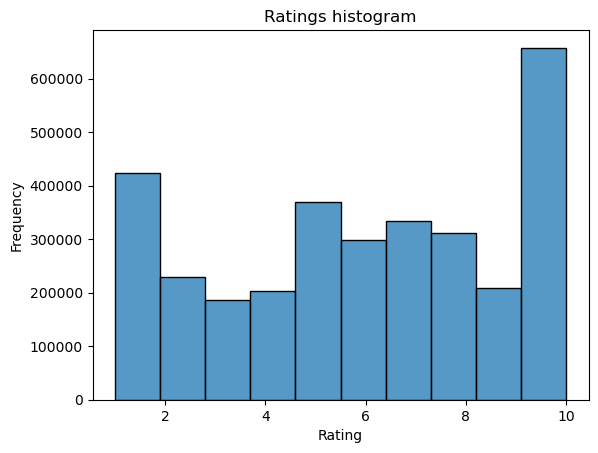
\includegraphics[width=0.6\linewidth]{figures/hist.png}
  \caption{Histogram of Profile Ratings}
  \label{fig:hist-rating}
\end{figure}

\subsubsection*{User Activity}
\begin{table}[H]
    \centering
    \caption{Number of Ratings Given per User}
    \label{tab:user-stats}
    \begin{tabular}{@{}lrrrrrrrr@{}}
    \toprule
    Statistic        & Count    & Mean    & Std     & Min & 25\% & 50\% & 75\%   & Max     \\ 
    \midrule
    Ratings per user & 25{,}245 & 127.55  & 362.10  & 2   & 29   & 73   & 123    & 18{,}342 \\
    \bottomrule
    \end{tabular}
\end{table}


\subsubsection*{Outlier Detection}
Using the IQR method ($Q_1 - 1.5\cdot\mathrm{IQR}$, $Q_3 + 1.5\cdot\mathrm{IQR}$), \emph{no} ratings fell outside the acceptable range, indicating the absence of extreme outliers.

\subsubsection*{Correlation Analysis}
We computed the Pearson correlation between the total number of ratings a profile received and its average rating:
\[
  \mathrm{Corr}(\text{rating\_count},\,\text{avg\_rating})
  \;=\;0.0201,
\]
a very weak positive relationship. The corresponding scatter plot (Figure~\ref{fig:rating-vs-count}) shows no strong trend.

\begin{figure}[H]
  \centering
  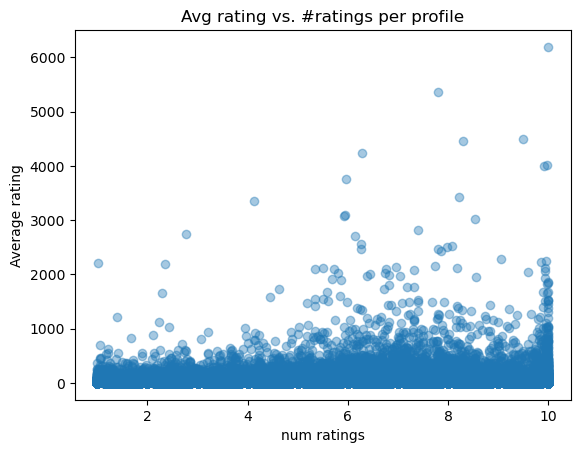
\includegraphics[width=0.6\linewidth]{figures/output.png}
  \caption{Average Rating vs.\ Number of Ratings per Profile}
  \label{fig:rating-vs-count}
\end{figure}